
\item From point \( A \) located on a highway (Fig. 1.2) one has to get by car as soon as possible to point \( B \) located in the field at a distance \( l \) from the highway. It is known that the car moves in the field \( \eta \) times slower than on the highway. At what distance from point \( D \) one must turn off the highway?
    \begin{center}
        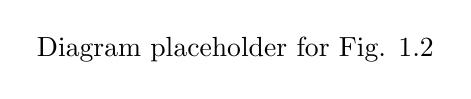
\begin{tikzpicture}
            \node at (0, 0) {Diagram placeholder for Fig. 1.2};
            % The actual TikZ commands for the diagram should go here
        \end{tikzpicture}
    \end{center}
    % Since there are no subquestions in the text provided, I am not including an enumerate environment. Should there be subquestions, the following template can be used:
    % \begin{enumerate}
    %     \item This is a subquestion.
    %     \item This is another subquestion.
    % \end{enumerate}
